
\chapter{Grundlagen der Programmierung}
\label{c:grundlagen}
\setcounter{page}{1}
\subsubsection{Was ist Progrmamieren?}

Schauen wir zunächsteinmal, wie einige der „großen Köpfe“ der
Informatik das Programmieren definieren.

\begin{quote}
	„To program is to understand“ \\
	\textit{~ Kristen Nygaard}
\end{quote}

\begin{quote}
	„Programming is a Good Medium for Expressing Poorly
	Understood and Sloppily Formulated Ideas“\\
	\textit{~ Marvin Minsky, Gerald J. Sussman}
\end{quote}

\section{Strukturierungsmechanismen}

\subsection{... einer Programmiersprache}

Eine Programmiersprache ist mehr als ein Hilfsmittel um einen Computer anzuweisen, Aufgaben durchzuführen.
Sie dient auch als \textbf{Rahmen}, innerhalb dessen wir \textbf{unsere Ideen} über die \textbf{Problemdomäne organisieren.}

Wenn wir eine Sprache beschreiben, sollten wir die Hilfsmittel beachten, die sie uns zum Kombinieren von einfachen Ideen anbietet, um komplexere Ideen zu bilden.

Jede vollwertige Programmiersprache hat drei Mechanismen, um Prozessideen zu strukturieren:

\subsection{... in der Informatik}

Zum einen \textbf{\textit{Primitive} Ausrücke}, welche die einfachsten Einheiten der Sprache repräsentieren. In der deutschen Sprache wäre zB. jedes Wort ein primitiver Ausdruck.

Ein weiterer sind die \textbf{\textit{Kombinationsmittel}}. Hier werden zusammengesetzte Elemente aus einfacheren Einheiten konstruiert. In der deutschen Sprache wäre dies eine zusammensetzung mehrerer Wörter zu einem Satz.

In der deutschen Sprache wären für \textbf{\textit{Abstraktionsmittel}} zB. die Definition eines Begriffs („Ein Auto ist ...“), so dass der Begriff danach als „Kurzform“ für die Erklärung nutzbar ist. Das gleiche geht natürlich auch in einer Programmiersprache. Hier können Zusammengesetzte Elemente benannt und weiter als Einheiten manipuliert werden

\subsection{... in der Elektronik}

In der Elektronik sind \textbf{\textit{Primitive} Ausrücke} zB. Widerstände, Kondensatoren, Induktivitäten, Spannungsquellen, usw...
\textbf{\textit{Kombinationsmittel}} wären in der Elektronik Richtlinien für das Verdrahten der Schaltkreise oder auch Standardschnittstellen (z.B. Spannungen, Strömungen) zwischen den Elementen. Diese Schnittstellen können auch Anforderungen an konkrete zulässige Werte oder Einheiten stellen („5 mA“)

Ein {\textit{Abstraktionsmittel}} wäre hier die “Black box” Abstraktion. Man betrachtet hier über einen Unter-Schaltkreis als eine Einheit: z.B. Verstärker, Regler, Empfänger, Sender, usw...

\section{Sprachelemente}

\subsection{Die Primitiven}
\subsubsection{Zahlen}
Zahlen sind selbstauswertend: Die Werte der Zifferfolge ist die Zahl, die sie bezeichnen.
$$ 23 \Rightarrow 23 $$
$$ -36 \Rightarrow -36 $$

\subsubsection{Boolesche Werte}
Boolsche Werte können nur \textit{wahr} oder \textit{falsch} sein. Diese sind ebenfalls
selbstauswertend. Sie werden als
$$ True \text{ oder } False $$
bezeichnet.
\subsubsection{Prozeduren}
Prozeduren sind in der Programmierung auch als „Funktionen“ oder „Methoden“ bekannt. Beispiele für eingebaute Prozeduren sind
$$ +, \; *, \; /, \; -, \; =, \; usw.$$
Aber was ist der Wert von so einem Ausdruck? Der Wert von + ist eine Prozedur, die Zahlen addiert. Dies werden wir später als „Higher-Order Procedures“ kennen lernen. Eine Auswertung bedeutet soviel wie das \textit{Nachschlagen} des dem Namen zugewiesenen Wertes.

\subsection{Besonderheiten bei Zahlen}
DrRacket rechnet immer genau, wenn dies möglich ist. Ganze und endliche Zahlen berechnet er so wie es „üblich ist“. Brüche mit periodischem Ergebnis werden ebenfalls in einem Text als Bruch - etwa \fbox{\textit{7/3}} dargestellt. Im Programm werden sie jedoch als Periode angezeigt. Beispielsweise \fbox{- 2.\uline{3}}. Doch kann nicht jede Zahl \textit{exakt} dargestellt werden. Man wird hier durch die Verwendung des Binärsystems eingeschränkt. Es gilt:
\begin{quote}
	„je mehr Nachkommastellen die Zahl besitzt, desto ungenauer wird in der Regel ihre Darstellung im Binärsystem“
\end{quote}

Zahlen unendlicher Länge ohne Periode werden wie folgt dargestellt: \fbox{\#i „inexact“}\\
Hier einige Beispiele:
$$e: \fbox{\#i2.718281828459045}$$
$$pi: \fbox{\#i3.141592653589793}$$
$$\sqrt{2}: \fbox{\#1.4142135623730951}$$

Mit Brüchen oder „inexakten“ Zahlen kann normal gerechnet
werden – das Ergebnis ist aber ggf. wieder „inexact“
$$(\sqrt{2})^2 = \fbox{\#i2.0000000000000004}$$

\subsection{Kombination}
Der Wert einer Kombination wird bestimmt durch die Ausführung der (durch den Operator) angegebenen Prozedur mit den Werten der Operanden. In Racket ist eine Sequenz von Ausdrücken eingeschlossen in Klammern. Die Ausdrücke sind primitiv oder erneut zusammengesetzt.

Hier ein Beispiel:
Numerische Ausdrücke können mit Ausdrücken kombiniert werden, die primitive Prozeduren repräsentieren (z.B. + oder *), um einen zusammengesetzten Ausdruck zu erstellen. Kombinationen können verschachtelt werden. Dafür müssen sie die Regeln einfach Rekursiv anwenden.
\begin{figure}
	\begin{center}
		
\includegraphics[height=2cm]{Bilder/T01_Sprachelemente_Kombination}
		\caption{}\label{t01_sk}
	\end{center}
\end{figure}

\begin{lstlisting}{t01-prog1}
(+ 4 (* 2 3)) = (4 + (2 * 3)) = 10
(* (+ 3 4) (- 8 2))
= ((3 + 4) * (8 - 2))
= 42
\end{lstlisting}

WICHTIG:
 Eine Kombination bedeutet immer eine Anwendung einer Prozedur. Klammern können nicht eingefügt oder weggelassen werden, ohne die Bedeutung des Ausdrucks zu ändern.

\subsection{Abstraktion}

In der Abstraktion wird zunächst erst etwas komplexes aus primitiven \textit{Bausteinen} gebaut. Dies wiederum wird nun benannt und kann daraufhin wieder als primitiver \textit{Baustein} behandelt werden. In Racket ist das einfachste Abstraktionsmittel das \fbox{define}. Im folgenden zwei Beispiele

\begin{lstlisting}{t01-prog2}
(define score (+ 27 3))
(define pi 3.14)
\end{lstlisting}

\textbf{Sonderformen} davon sind geklammerte Ausdrücke, die mit einem wenigen HtDP-TL-Schlüsselwörter starten. Ein Beispiel hierfür wäre \fbox{define}.  Mit define kann man einen Wert an einen Namen binden wie im zuvor genannten Beispiel sichtbar. Die \fbox{define} Sonderform wertet den zweiten Ausdruck nicht aus (in diesem Beispiel: \fbox{score}). Sie assoziiert diesen Namen mit dem Wert des dritten Ausdruckes in einer Umgebung. \fbox{define} liefert keinen Wert als Ergebnis der Auswertung. Wir sehen: \fbox{define} liefert keinen Wert als Ergebnis der Auswertung.

\subsection{Namensgebung und Umgebung}
Ein wichtiger Aspekt einer Programmiersprache ist die Möglichkeit, Objekte über Namen zu referenzieren.  Ein Name identifiziert eine Variable, deren Wert ein Objekt ist. Das Objekt kann dabei ein primitiver Ausdruck sein (z.B. Zahlen) oder  beliebig komplex, z.B. eine Struktur ($\Rightarrow$ T02) oder Liste ($\Rightarrow$ T03).\\

Der Interpreter unterhält eine Art Speicher, um Name-Objekt Paare zu verwalten. Darin werden die Werte mit den hinterlegten Symbolen bzw. Namen assoziiert. So können später dann die Werte über die Symbole dann zugewiesen werden. Man kann sich die \textit{Umgebung} wie ein Telefon- oder Wörterbuch vorstellen. Hinter jedem Namen steht also das damit verknüpfte Objekt (statt einer Telefonnummer bzw. Definition).

Um den Wert auszurechnen, der durch den Namen repräsentiert wird, reicht es aus, ihn in der Umgebung aufzulösen. Als Beispiel: Die Evaluierung von score ist 30

Hierbei ist zu beachten: Wir haben das alles für die Symbole der arithmetischen Operatoren +, *, usw. schon vorausgesetzt. Man muss sich also nicht damit beschäftigen \textit{wie} sie funktionieren. Es reicht nur zu wissen \textit{was} sie machen.

\subsection{Auswertungsregel}
Ein Ausdruck der \textit{Selbst-auswertend (self-rule)} ist, ist zB. eine Zahl. Der Wert des primitiven Ausdrucks 42 ist die Zahl 42.

Ein \textit{Eingebauter Operator} gibt die Sequenz der Maschineninstruktionen zurück, die die entsprechenden Operationen durchführen.

Ein \textit{Name (name-rule)} gibt den Wert zurück, der in der Umgebung mit diesem Namen assoziiert wurde.

Eine \textit{Sonderform} macht etwas "Besonderes".

Eine \textit{Kombination} wertet die Unterausdrücke zunächst (in beliebiger Reihenfolge) aus. Daraufhin wird die Prozedur, die der Wert des am weitesten links liegenden Unterausdruckes ist (der Operator), auf die Argumente (die Werte der restlichen Unterausdrücke (Operanden)) angewendet.
Beispiel einer Kombination: \fbox{(+ 4 (* 2 3))}

Die \textit{Auswertungsregel} ist rekursiv. Das heißt bei einer Kombination ruft die Regel sich selbst auf. Auch muss jedes Element ausgewertet werden, bevor die Gesamtauswertung einer Kombination abgeschlossen werden kann.

Die Auswertung der folgenden Kombination erfordert die Anwendung der Auswertungsregel auf vier unterschiedliche Kombinationen.

 \fbox{(* \fbox{(+ 2 \fbox{(* 4 6)} )} \fbox{(+ 3 5 7)})}

In der \fbox{define}-Regel wird nur der zweite Operand ausgewertet. Der Name ist hier nur an den berechneten Wert gebunden. Somit ist der Gesamtwert des Ausdrucks undefiniert.
\begin{lstlisting}{t01-prog3}
(define pi 3.14)
\end{lstlisting}
\fbox{\fbox{Name $\Rightarrow$ pi} \fbox{Wert $\Rightarrow$ 4.14}} \\

Bei einer Zahl ist das ganze ein wenig einfacher. Wenn wir nun \textit{23} in den Interpreter eintippen gilt zunächst die \textit{self-rule} und der Ausdruck \textit{23} ist somit selbstauswertend. In der Ausgabe wird also auch \textit{23} ausgegeben.

\fbox{\fbox{Ausdruck $\Rightarrow$ 23} \fbox{Wert $\Rightarrow$ 23} \fbox{Ausgabe $\Rightarrow$ 23}}\\

Geben wir nun aber \textit{pi} ein gilt die \textit{name-rule}.

\fbox{\fbox{Ausdruck $\Rightarrow$ pi} \fbox{Wert $\Rightarrow$ 3.14} \fbox{Ausgabe $\Rightarrow$ 3.14}}

\subsection{Definition neuer Prozeduren}
Im folgenden sehen wir drei verschiedene Beispiele einer Kresiflächenberechnung und wir stellen Fest, dass alle Berechnungen ein gleiches Muster haben. Wir sollten uns jetzt fragen, wie wir es schaffen dieses Muster zu generalisieren.
\begin{lstlisting}{t01-prog4}
(* 3.14 (* 5 5))
(* 3.14 (* 23.2 23.2))
(* 3.14 (* r r))
\end{lstlisting}
Um wiederkehrende Muster festzuhalten benutzen wir \textit{Prozeduren}. Diese sind analog zu einer Funktionsdefinition in der Mathematik. Deshalb geben wir ihnen auch manchmal den gleichen Namen \textit{Funktion}. Um neue Prozeduren zu definieren verwenden wir die \fbox{define}-Sonderform. (siehe Abbildung \ref{fig:t01_pd})

\begin{figure}
  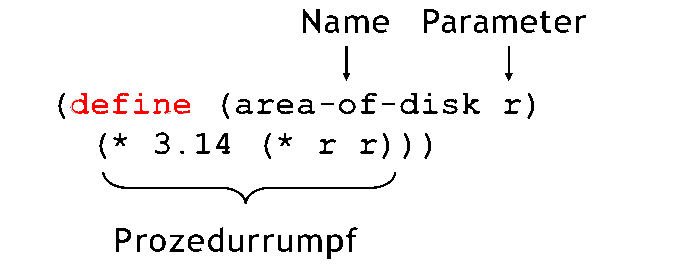
\includegraphics[height=4cm]{Bilder/T01_def_newproc.png}
  \caption{Prozedur Definition}
  \label{fig:t01_pd}
\end{figure}

Sobald eine Prozedur definiert wurde, kann sie wie eine
primitive Prozedur (wie +, * etc.) benutzt werden.
\begin{lstlisting}{t01-prog5}
(area-of-disk 5)
	;; -> ergibt 78.5
(- (area-of-disk 5) (area-of-disk 3))
	;; -> ergibt (78.5 - 28.26) = 50.24
\end{lstlisting}
Bereits definierte Prozeduren können auch zu neuen Prozeduren
kombiniert werden.
\begin{lstlisting}{t01-prog5}
(define (area-of-ring outer inner)
	(- (area-of-disk outer) (area-of-disk inner)))
\end{lstlisting}
Die Anwendung sähe wie folgt aus:
\begin{lstlisting}{t01-prog5}
(area-of-ring 5 3)
	;; = (- (area-of-disk 5) (area-of-disk 3))
	;; = (- (* 3.14 (* 5 5)) (* 3.14 (* 3 3)))
	;; = ... = 50.24
\end{lstlisting}

\subsection{Informelle Beschreibungen}
Eine informelle Beschreibungen sind üblicherweise nicht in Form mathematischer Ausdrücke geschrieben. Sie sind informelle Problembeschreibungen, welche in Programmeumzuwandeln sind. Meist enthalten sie auch irrelevante oder mehrdeutige Informationen.

\subsubsection{Beispiel}
\textit{Die Firma XYZ bezahlt ihren Angestellten 12 € pro Stunde. Ein Angestellter arbeitet zwischen 20 und 65 Stunden pro Woche. Entwickeln Sie ein Programm, welches den Lohn eines Angestellten aus der Anzahl der Arbeitsstunden berechnet.}
\begin{lstlisting}{t01-prog6}
(define (lohn stundenanzahl)
	(* 12 stundenanzahl))
\end{lstlisting}

\subsection{Fehler}
Ihre Programme werden meist Fehler enthalten. Jedoch ist dies nichts Schlimmes. Lassen Sie sich durch Fehler nicht verwirren oder entmutigen. Sowas gehört dazu. :)
Mögliche Fehler wären zB. diese:
\begin{lstlisting}{t01-prog6}
;; Falsche klammerung
(* 3 (5)
;; Operator eines Prozeduraufrufs ist keine Prozedur
(10)
(10 + 20)
;; Typfehler und andere Laufzeitfehler
(+ 3 true)
(/ 3 0)
\end{lstlisting}
Probieren Sie einmal aus, was bei fehlerhaften Eingaben passiert und versuchen Sie die Fehlermeldungen zu verstehen!

\subsection{Design von Programmen}
Das Design von Programmen ist nicht trivial. Das folgende Rezept soll Ihnen helfen, Ihre ersten Programme zu schreiben. Es wird im folgenden eine "Schritt für Schritt Beschreibung" gegeben, was zu tun ist und wie sie vorgehen können. Später wird dieses Rezept noch ein wenig verfeinert.

\subsubsection{Jede Programmentwicklung besteht aus
mindestens den folgenden vier Aktivitäten:}

\begin{itemize}
	\item Verstehen, was der Zweck des Programms ist
	\item Nutzungsbeispiele ausdenken
	\item Den Programmkörper implementieren
	\item Testen
\end{itemize}

\begin{quote}
	„If you can't write it down in English, you can't code it.	“ \\
	\textit{~ Peter Halpern}
\end{quote}

\subsubsection{Verstehen, was der Zweck des Programms ist:}
Vergeben sie zunächst einen sinnvollen \textit{Namen} und definieren sie darauf hin einen \textit{Vertrag}. In diesen Vertrag wird beschrieben welche Arten von Daten verarbeitet („konsumiert“) und welche werden als Ergebnis geliefert („produziert“) werden.
\begin{lstlisting}{t01-prog7}
;; area-of-ring :: number number -> number
;; Berechnet die Flaeche eines Rings
;; mit Radius "outer", dessen
;; Loch den Radius "inner" hat
\end{lstlisting}

\subsubsection{Nutzungsbeispiele ausdenken}
Nutzungsbeispiele helfen die Ein-/Ausgaberelation zu charakterisieren. Es ist oft einfacher, Abstraktes anhand von Beispielen zu verstehen und logische Fehler zu entdecken.

\begin{lstlisting}{t01-prog7}
;; Beispiel: (area-of-ring 5 2) ergibt 65.94
\end{lstlisting}

\subsubsection{Implementierung}
Ist die Eingabe-Ausgabe Relation eine mathematische Formel, können wir diese meist direkt übersetzen.  Bei einer informellen Beschreibung müssen wir uns den Berechnungsprozess klarmachen. Hierbei können die Beispiele aus Schritt 2 helfen.

\begin{lstlisting}{t01-prog7}
(define (area-of-ring outer inner)
	(- (area-of-disk outer) (area-of-disk inner)))
\end{lstlisting}

\subsubsection{Testen!}
\begin{quote}
	“Testing can show the presence of bugs, but not their absence.”\\
	\textit{~ Edsger W. Dijkstra}
\end{quote}
\begin{quote}
	“Beware of bugs in the above code; I have only proved it correct, not tried it“\\
	\textit{~ Donald E. Knuth}
\end{quote}

Nutzen Sie die folgenden eingebauten Prozeduren der HtDP-TL um ihren Programmcode auf Bugs zu untersuchen.
\begin{lstlisting}{t01-tests}
;; Vergleicht den “test"-Wert exakt mit
;; dem "expected"-Wert
(check-expect test expected)

;; Prüfung, ob der Testwert (meist Gleitkommazahl)
;; korrekt ist mit Abweichung ± delta, etwa delta = 0.0001.
(check-within test expected delta)

;; Prüft, ob der Aufruf die erwartete Fehlermeldung liefert
(check-error test message)
\end{lstlisting}

% TODO Hilfsprozeduren
% TODO Blackbox
\subsection{Bedingte Ausdrücke}
In der HtDP-TL gibt es zwei Formen von bedingten Ausdrücken.
\begin{lstlisting}{t01-if}
;; Form 1)
(if <test>
	<then-expr>
	<else-expr>) ;; in HtDP-TL nicht optional!

;; Form 2)
(cond
	[<test1> <expr1>]
	[<test2> <expr2>]
	. . .
	[else <last-expr>]) ;; optional
\end{lstlisting}

\subsection{Boolsche Funktionen}
\begin{lstlisting}{t01-bool}
(and <expr_1> <expr_2> . . . <expr_N>)
;; Beispiele:
(and (= 4 4) (< 5 3))
(and true (+ 3 5))
	;;-> false
 	;; Fehler: and: question result is not true or false: 8
(and false (+ 3 5))
	;; -> Shortcut-Regel: false
\end{lstlisting}
\fbox{<expr\_i> (i = 1..N)} werden in dieser Reihenfolge ausgewertet. Es wird \textit{false} zurück gegeben, falls irgendein Ausdruck als \textit{false} ausgewertet wird, sonst wird \textit{true} zurückgegeben. Wenn einer der ausgewerteten Ausdrücke weder tru\textit{true} noch \textit{false} ergibt, gibt es einen Fehler. Durch Shortcut-Regel werden manche Ausdrücke nicht ausgewertet.

\begin{lstlisting}{t01-bool}
(or <expr1_> <expr_2> . . . <expr_N>)
\end{lstlisting}

\begin{lstlisting}{t01-bool}
(boolean=? <expr1> <expr2>)
\end{lstlisting}

\begin{lstlisting}{t01-bool}
(not <expr>)
\end{lstlisting}

\subsection{Design konditionaler Prozeduren}
Jede Programmentwicklung besteht aus wenigstens vier Aktivitäten.
\begin{itemize}
	\item 1. Verstehen, was der Zweck des Programms ist
	\item 2.  Nutzungsbeispiele ausdenken
	\item 3.  Den Programmkörper implementieren
	\item 4.  Testen
\end{itemize}

Neue Phase: Datenanalyse
§  Welche unterschiedlichen Situationen gibt es?
§  Beispiele
§  Mindestens ein Beispiel für jede Situation
§  Implementierung des Programmkörpers
§  Erst Skelett der cond/if Ausdrücke definieren, dann die einzelnen
Fälle implementieren
§  Testen
§  Tests sollten alle Situationen abdecken

\subsubsection{Bitte Beachten!}
Überflüssigen Code vermeiden! Dieser Code...:
\begin{lstlisting}
(if (< x 0)
	true
	false)
\end{lstlisting}
... ist identisch zu:
\begin{lstlisting}
(< x 0)
\end{lstlisting}
Entsprechend bei „umgekehrter Logik“..
\begin{lstlisting}
(if (>= x 0)
	false
	true)
\end{lstlisting}
kürzer, klarer, besser
\begin{lstlisting}
(< x 0)
;; Alternative
(not (>= x 0))
\end{lstlisting}

% TODO
\subsection{Symbole}
Bis jetzt hatten wir Zahlen und Booleans als primitive Werte
kennengelernt
§  Oft wollen wir symbolische Informationen speichern
§  Namen, Wörter, Richtungen,...
§  Ein Symbol ist in HtDP-TL eine Sequenz von Zeichen, angeführt
von einem einfachen Anführungszeichen:
§  'the 'dog 'ate 'a 'cat! 'two^3 'and\%so\%on?
§  Nicht alle Zeichen sind erlaubt (z.B. keine Leerzeichen)
§  Nur eine Operation auf diesem Datentyp: \fbox{symbol=?

\begin{lstlisting}
(symbol=? 'Hallo 'Hallo) -> true
(symbol=? 'Hallo 'ABC) -> false
(symbol=? 1 2) -> Fehler
\end{lstlisting}

Symbole sind atomar (wie auch Zahlen, Booleans) dh. Symbole können nicht zerlegt werden.

\begin{lstlisting}
;; reply: symbol -> symbol
;; give a decent reply to a greeting or questions
;; example: (reply 'GoodMorning) is 'Hi
(define (reply s)
	(cond
		[(symbol=? s 'GoodMorning) 'Hi]
		[(symbol=? s 'HowAreYou?) 'Fine]
		[(symbol=? s 'GoodAfternoon) 'INeedANap]
		[(symbol=? s 'GoodEvening) 'BoyAmITired]
		[else (error 'reply "unknown case")] ))
;; Tests
(check-expect (reply 'GoodMorning) 'Hi)
(check-expect (reply 'HowAreYou?) 'Fine)
\end{lstlisting}
